\documentclass[tikz,border=3mm]{standalone}
\usepackage{booktabs}
\usepackage{amsmath}
\usepackage{xcolor}
\usepackage{colortbl}

\begin{document}

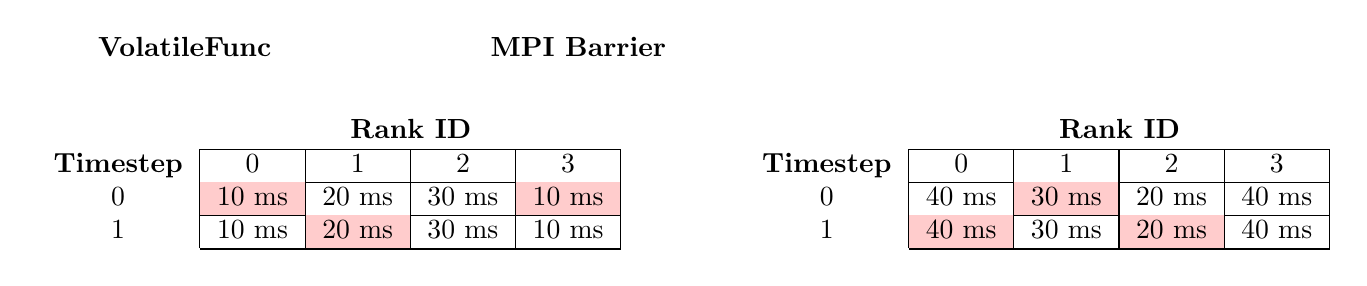
\begin{tikzpicture}

% VolatileFunc Title
\node[anchor=north] at (2, 1) {\textbf{VolatileFunc}};

% VolatileFunc Duration Matrix with highlights
\node[anchor=north west] at (0, 0) {
\begin{tabular}{c|c|c|c|c|}
\multicolumn{1}{c}{} & \multicolumn{4}{c}{\textbf{Rank ID}} \\ \cline{2-5}
\textbf{Timestep} & 0 & 1 & 2 & 3 \\ \cline{2-5}
0                & \cellcolor{red!20}10 ms & 20 ms & 30 ms & \cellcolor{red!20}10 ms \\ \cline{2-5}
1                & 10 ms & \cellcolor{red!20}20 ms & 30 ms & 10 ms \\ \cline{2-5}
\end{tabular}
};

% MPI_Barrier Title
\node[anchor=north] at (7, 1) {\textbf{MPI Barrier}};

% MPI_Barrier Duration Matrix with highlights
\begin{scope}[xshift=4cm]
\node[anchor=north west] at (5, 0) {
\begin{tabular}{c|c|c|c|c|}
\multicolumn{1}{c}{} & \multicolumn{4}{c}{\textbf{Rank ID}} \\ \cline{2-5}
\textbf{Timestep} & 0 & 1 & 2 & 3 \\ \cline{2-5}
0                & 40 ms & \cellcolor{red!20}30 ms & 20 ms & 40 ms \\ \cline{2-5}
1                & \cellcolor{red!20}40 ms & 30 ms & \cellcolor{red!20}20 ms & 40 ms \\ \cline{2-5}
\end{tabular}
};
\end{scope}

\end{tikzpicture}

\end{document}